\documentclass[a4paper, 12pt]{article}
\usepackage[a4paper,top=1.5cm, bottom=1.5cm, left=1cm, right=1cm]{geometry}

% Работа с русским языком
\usepackage[utf8]{inputenc}
\usepackage{mathtext}                % русские буквы в формулах
\usepackage[english, russian]{babel} % локализация и переносы

\usepackage{graphicx}   % Вставка изображений
\usepackage{float}      % "Плавающие" изображения3
\usepackage{wrapfig}    % Обтекание фигур (таблиц, картинок и прочего)
\graphicspath{ {./images/} }

\usepackage{tabularx}
\usepackage{multirow}
\usepackage{amsmath}
\usepackage{amsfonts}
\usepackage{indentfirst}
\usepackage{longtable}
\graphicspath{{pictures/}}
\usepackage{natbib}
\usepackage{bm}

%%% Колонтитулы
\usepackage{titleps}
\newpagestyle{main}{
	\setheadrule{0.4pt}
	\sethead{Эффект Холла в полупроводниках}{}{}
	\setfootrule{0.4pt}                       
	\setfoot{ФРКТ МФТИ, 2023}{}{\thepage} 
}
\pagestyle{main}  

\begin{document}
    \begin{titlepage}
	\begin{center}
            {\large МОСКОВСКИЙ ФИЗИКО-ТЕХНИЧЕСКИЙ ИНСТИТУТ (НАЦИОНАЛЬНЫЙ ИССЛЕДОВАТЕЛЬСКИЙ УНИВЕРСИТЕТ)}
	\end{center}
 
	\begin{center}
		{\large Физтех-школа радиотехники и компьютерных технологий}
	\end{center}
	
	\vspace{8cm}
	{\LARGE
		\begin{center}
                {\bf Отчёт о выполнении лабораторной работы 3.3.4}\\
                Эффект Холла в полупроводниках
		\end{center}
	}
	\vspace{5cm}
	\begin{flushright}
		{\Large Автор:\\ Тихонов Дмитрий Романович, \\
			\vspace{0.2cm}
			студент группы Б01-206}
	\end{flushright}
	\vspace{5cm}
	\begin{center}
		\Large Долгопрудный, 2023
	\end{center}
    \end{titlepage}

    \section{Введение}

    \noindent \textbf{Цель работы:} измерение подвижности и концентрации носителей заряда в полупроводниках. \\

    \noindent \textbf{В работе используются:} электромагнит с источником питания GPR, батарейка 1,5 В, амперметр, реостат, цифровой вольтметр В7-78/1, милливеберметр, образцы легированного германия.
    
    \section{Теоретические сведения}

    Движение электронов в некоторой кристаллической решётке под действием внешнего электрического поля можно описать следующей формулой:

    \begin{equation}
        \langle \bm{v} \rangle = -b \bm{E},
    \end{equation}

    где $\langle \bm{v} \rangle$ -- некоторая средняя скорость электронов, а $b$ -- величина, называемая \textit{подвижностью электронов}.

    Плотность тока равна

    \begin{equation}
        j = e n \langle v \rangle = enbE.
    \end{equation}

    Отсюда, находим выражение для проводимости:

    \begin{equation}
        \sigma = enb.
    \end{equation}

    Если в проводнике присутствует внешнее магнитное поле $\bm{B}$, то на электроны действует сила Лоренца, равная

    \begin{equation}
        \bm{F_\text{Л}} = -e \left( \bm{E} + \langle \bm{v} \rangle \times \bm{B} \right)
    \end{equation}

     \begin{wrapfigure}{r}{6cm}
	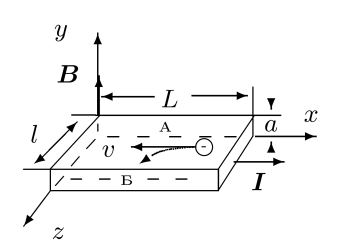
\includegraphics[width=6cm]{images/theor.png}
	\caption{Образец с током в магнитном поле}
	\label{theor}
    \end{wrapfigure}

    Рассмотрим проводник с током в форме прямоугольного параллелепипеда со сторонами $L$, $a$ и $l$, параллельными осям $x$, $y$ и $z$ соответственно, в котором течет ток $I$ вдоль оси $x$ (рис. \ref{theor}).

    Пусть поле $\bm{E}$ направлено против оси $x$, поле $\bm{B}$ -- вдоль оси $y$. Тогда дрейфовая скорость электронов будет направлена против оси $x$ и часть силы Лоренца, зависящая от магнитного поля, направлена вдоль оси $z$ и равна

    \begin{equation}
        F_B = ebEB
    \end{equation}

    Эта сила заставляет электроны смещаться в направлении оси $z$. Из-за этого в установившемся режиме возникает противоположно направленное поле $E_z$, компенсирующее силу $F_B$:

    \begin{equation}
        E_z = bEB = \frac{bjB}{\sigma} = \frac{IB}{enS} = \frac{IB}{e \cdot n \cdot al}
    \end{equation}
    
    Поле $E_z$ создаёт ЭДС Холла, равную

    \begin{equation}\label{1}
        \mathcal{E}_x = \frac{IB}{nea} = - R_x \cdot \frac{IB}{a},
    \end{equation}

    Константа $R_x$ называется \textit{постоянной Холла} и равна

    \begin{equation}
        \label{eq_Rx}
        R_x=\frac{1}{ne}.
    \end{equation}
    
    \section{Методика измерений и используемое оборудование}

    Электрическая схема установки для измерения ЭДС Холла представлена на рис. \ref{installation}.

    \begin{figure}[H]
        \centering
        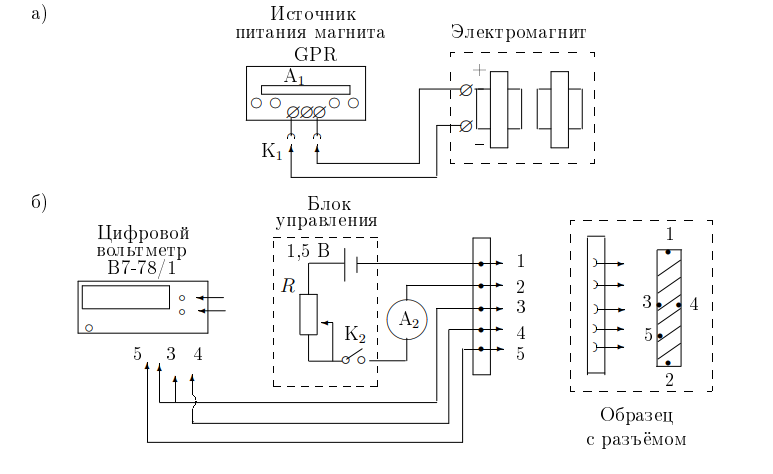
\includegraphics[width = 15 cm]{images/installation.png}
        \caption{Схема установки для исследования эффекта Холла в полупроводниках}
        \label{installation}
    \end{figure}

    В зазоре электромагнита (рис. \ref{installation}а) создается постоянное магнитное поле, величину которого можно менять с помощью регуляторов источника питания. Ток измеряется амперметром источника питания $А_1$. Разъём $K_1$ позволяет менять направление тока в обмотках электромагнита. Градуировка магнита проводится при помощи милливеберметра.
    
    Образец из легированного германия, смонтированный в специальном держателе (рис. \ref{installation}б), подключается к батарее. При замыкании ключа $К_2$ вдоль длинной стороны образца течёт ток, величина которого регулируется реостатом $R$ и измеряется миллиамперметром $А_2$. 
    
    В образце с током, помещённом в зазор электромагнита, между контактами $3$ и $4$ возникает разность потенциалов $U_{34}$, которая измеряется с помощью цифрового вольтметра. Контакты $3$ и $4$ вследствие неточности подпайки не всегда лежат на одной эквипотенциали, и тогда напряжение между ними связано не только с эффектом Холла, но и с омическим падением напряжения, вызванным протеканием основного тока через образец. Исключить влияние омического падения напряжения можно, если при каждом токе через образец измерять напряжение между точками $3$ и $4$ в отсутствие магнитного поля. При фиксированном токе через образец это дополнительное к ЭДС Холла напряжение $U_0$ остаётся неизменным. От него следует отсчитывать величину ЭДС Холла с учётом знака: = $U_{34} \pm U_0$. При таком способе измерения нет необходимости проводить повторные измерения с противоположным направлением магнитного поля.
    
    По знаку можно определить характер проводимости - электронный или дырочный. Для этого необходимо знать направление тока в образце и направление магнитного поля.
    
    Измерив ток в образце и напряжение $U_{35}$ между контактами $3$ и $5$ в отсутствие магнитного поля, можно, зная параметры образца, рассчитать проводимость материала образца по очевидной формуле:

    \begin{equation}
        \sigma = I \cdot L_{35} / \left( U_{35} \cdot a \cdot l \right), 
        \label{eq_sigma}
    \end{equation}
    
    где $L_{35}$ -- расстояние между контактами 3 и 5, $а$ -- толщина образца, $l$ -- его ширина.

    \section{Результаты измерений и обработка данных}

    \subsection{Градуировка электромагнита}
    
    Была исследована зависимость индукции $\Delta \Phi$ магнитного поля в зазоре электромагнита от тока через обмотки магнита. Для вычисления индукции $В$ была применена формула

    \begin{equation}
        B = \frac{\Delta \Phi}{SN},
    \end{equation}

    где $\Delta \Phi$ - разность между начальным и конечным значением потока вектора индукции, который пронизывал пробную катушку, находившуюся в зазоре электромагнита, а $SN = 75 \: \text{см}^2 \cdot \text{вит}$.
    
    Результаты измерений представлены в таблице \ref{graduation}. По этим данным построим график зависимости $B = f(I_\text{М})$ (рис. \ref{graph:graduation}).

    \begin{table}[H]
        \centering
        \begin{tabular}{|c|c|c|}
        \hline
        $I_\text{М}$, А & $\Delta \Phi$, мВб & $B$, Тл \\ \hline
        0,19 & 1,0 & 0,13 \\ \hline
        0,39 & 1,9 & 0,25 \\ \hline
        0,60 & 2,8 & 0,37 \\ \hline
        0,80 & 3,7 & 0,49 \\ \hline
        1,00 & 4,5 & 0,60 \\ \hline
        1,20 & 5,1 & 0,68 \\ \hline
        1,60 & 6,1 & 0,81 \\ \hline
        1,80 & 6,5 & 0,87 \\ \hline
        2,00 & 6,8 & 0,91 \\ \hline
        2,12 & 6,9 & 0,92 \\ \hline
        \end{tabular}
        \caption{Результаты измерения зависимости $B = f(I_\text{М})$}
        \label{graduation}
    \end{table}

    \begin{figure}[H]
        \centering
        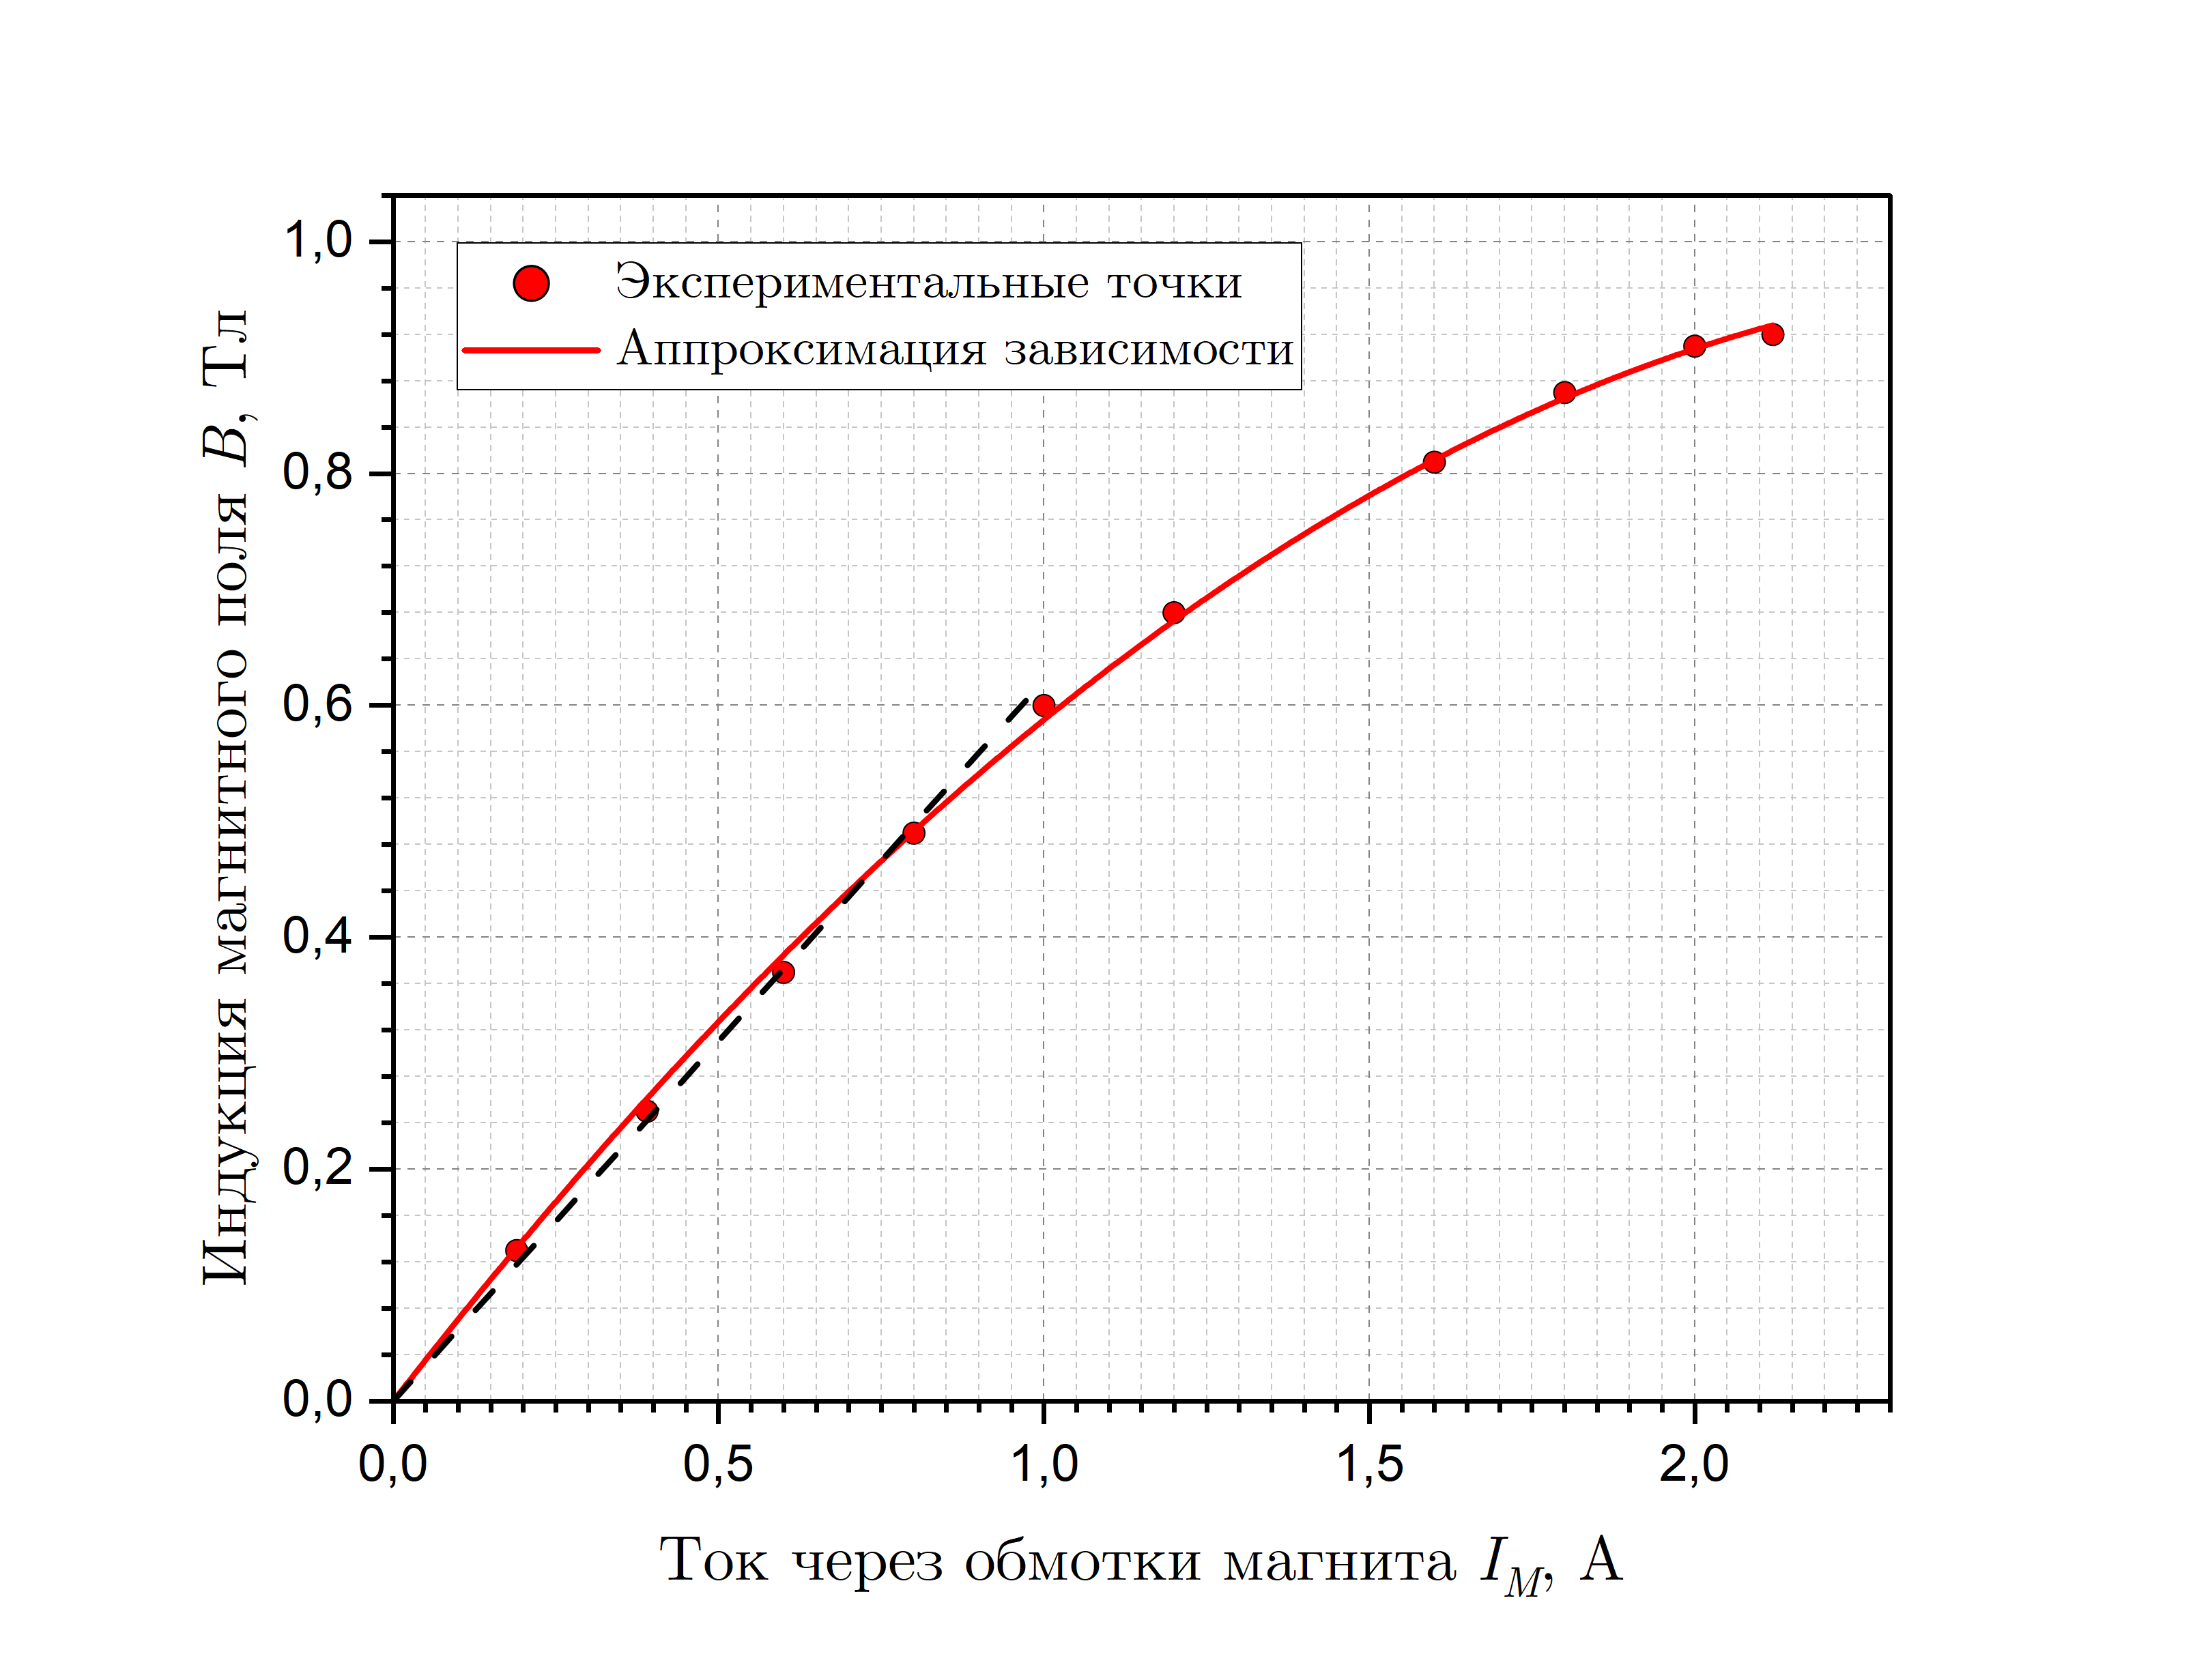
\includegraphics[width = 15 cm]{images/graph_graduation.png}
        \caption{График зависимости $B = f(I_\text{М})$}
        \label{graph:graduation}
    \end{figure}

    \subsection{Измерение ЭДС Холла}

    Была исследована зависимость напряжения $U_{34}$ от тока $I_\text{М}$ через обмотки магнита при фиксированном токе через образец. При этом в отсутствие магнитного поля вольтметр показывал напряжение $U_0$, которое также зависело от тока $I_\text{М}$. При расчёте ЭДС Холла использовалась формула

    \begin{equation}
        \mathcal{E}_x = U_{34} - U_0.
    \end{equation}
    
    При максимально возможном токе через образец измерение было проведено при изменённой ориентации образца. Результаты полученных значений представлены в таблице \ref{measurement_EMF_1}.

    \begin{table}[H]
        \centering
        \begin{tabular}{ccccccccc}
        \hline
        \multicolumn{3}{|c|}{$I = 0,3$ мА} & \multicolumn{3}{c|}{$I = 0,4$ мА} & \multicolumn{3}{c|}{$I = 0,5$ мА} \\ \hline
        \multicolumn{3}{|c|}{$U_0 = -17$ мкВ} & \multicolumn{3}{c|}{$U_0 = -23$ мкВ} & \multicolumn{3}{c|}{$U_0 = -29$ мкВ} \\ \hline
        \multicolumn{1}{|c|}{$I_M$, А} & \multicolumn{1}{c|}{$U_{34}$, мкВ} & \multicolumn{1}{c|}{$\mathcal{E}_x$, мкВ} & \multicolumn{1}{c|}{$I_M$, А} & \multicolumn{1}{c|}{$U_{34}$, мкВ} & \multicolumn{1}{c|}{$\mathcal{E}_x$, мкВ} & \multicolumn{1}{c|}{$I_M$, А} & \multicolumn{1}{c|}{$U_{34}$, мкВ} & \multicolumn{1}{c|}{$\mathcal{E}_x$, мкВ} \\ \hline
        \multicolumn{1}{|c|}{0,20} & \multicolumn{1}{c|}{-36} & \multicolumn{1}{c|}{-19} & \multicolumn{1}{c|}{0,20} & \multicolumn{1}{c|}{-47} & \multicolumn{1}{c|}{-24} & \multicolumn{1}{c|}{0,19} & \multicolumn{1}{c|}{-59} & \multicolumn{1}{c|}{-30} \\ \hline
        \multicolumn{1}{|c|}{0,57} & \multicolumn{1}{c|}{-70} & \multicolumn{1}{c|}{-53} & \multicolumn{1}{c|}{0,56} & \multicolumn{1}{c|}{-91} & \multicolumn{1}{c|}{-68} & \multicolumn{1}{c|}{0,58} & \multicolumn{1}{c|}{-117} & \multicolumn{1}{c|}{-88} \\ \hline
        \multicolumn{1}{|c|}{0,98} & \multicolumn{1}{c|}{-105} & \multicolumn{1}{c|}{-88} & \multicolumn{1}{c|}{1,05} & \multicolumn{1}{c|}{-146} & \multicolumn{1}{c|}{-123} & \multicolumn{1}{c|}{1,05} & \multicolumn{1}{c|}{-187} & \multicolumn{1}{c|}{-158} \\ \hline
        \multicolumn{1}{|c|}{1,39} & \multicolumn{1}{c|}{-133} & \multicolumn{1}{c|}{-116} & \multicolumn{1}{c|}{1,38} & \multicolumn{1}{c|}{-175} & \multicolumn{1}{c|}{-152} & \multicolumn{1}{c|}{1,42} & \multicolumn{1}{c|}{-224} & \multicolumn{1}{c|}{-195} \\ \hline
        \multicolumn{1}{|c|}{1,80} & \multicolumn{1}{c|}{-149} & \multicolumn{1}{c|}{-132} & \multicolumn{1}{c|}{1,78} & \multicolumn{1}{c|}{-197} & \multicolumn{1}{c|}{-174} & \multicolumn{1}{c|}{1,80} & \multicolumn{1}{c|}{-248} & \multicolumn{1}{c|}{-219} \\ \hline
        \multicolumn{1}{|c|}{2,12} & \multicolumn{1}{c|}{-158} & \multicolumn{1}{c|}{-141} & \multicolumn{1}{c|}{2,10} & \multicolumn{1}{c|}{-208} & \multicolumn{1}{c|}{-185} & \multicolumn{1}{c|}{2,09} & \multicolumn{1}{c|}{-261} & \multicolumn{1}{c|}{-232} \\ \hline
        \multicolumn{1}{l}{} & \multicolumn{1}{l}{} & \multicolumn{1}{l}{} & \multicolumn{1}{l}{} & \multicolumn{1}{l}{} & \multicolumn{1}{l}{} & \multicolumn{1}{l}{} & \multicolumn{1}{l}{} & \multicolumn{1}{l}{} \\ \hline
        \multicolumn{3}{|c|}{$I = 0,6$ мА} & \multicolumn{3}{c|}{$I = 0,7$ мА} & \multicolumn{3}{c|}{$I = 0,8$ мА} \\ \hline
        \multicolumn{3}{|c|}{$U_0 = -35$ мкВ} & \multicolumn{3}{c|}{$U_0 = -43$ мкВ} & \multicolumn{3}{c|}{$U_0 = -50$ мкВ} \\ \hline
        \multicolumn{1}{|c|}{$I_M$, А} & \multicolumn{1}{c|}{$U_{34}$, мкВ} & \multicolumn{1}{c|}{$\mathcal{E}_x$, мкВ} & \multicolumn{1}{c|}{$I_M$, А} & \multicolumn{1}{c|}{$U_{34}$, мкВ} & \multicolumn{1}{c|}{$\mathcal{E}_x$, мкВ} & \multicolumn{1}{c|}{$I_M$, А} & \multicolumn{1}{c|}{$U_{34}$, мкВ} & \multicolumn{1}{c|}{$\mathcal{E}_x$, мкВ} \\ \hline
        \multicolumn{1}{|c|}{0,22} & \multicolumn{1}{c|}{-75} & \multicolumn{1}{c|}{-40} & \multicolumn{1}{c|}{0,18} & \multicolumn{1}{c|}{-80} & \multicolumn{1}{c|}{-37} & \multicolumn{1}{c|}{0,19} & \multicolumn{1}{c|}{-93} & \multicolumn{1}{c|}{-43} \\ \hline
        \multicolumn{1}{|c|}{0,57} & \multicolumn{1}{c|}{-140} & \multicolumn{1}{c|}{-105} & \multicolumn{1}{c|}{0,57} & \multicolumn{1}{c|}{-165} & \multicolumn{1}{c|}{-122} & \multicolumn{1}{c|}{0,59} & \multicolumn{1}{c|}{-193} & \multicolumn{1}{c|}{-143} \\ \hline
        \multicolumn{1}{|c|}{0,98} & \multicolumn{1}{c|}{-211} & \multicolumn{1}{c|}{-176} & \multicolumn{1}{c|}{1,03} & \multicolumn{1}{c|}{-256} & \multicolumn{1}{c|}{-213} & \multicolumn{1}{c|}{1,02} & \multicolumn{1}{c|}{-300} & \multicolumn{1}{c|}{-250} \\ \hline
        \multicolumn{1}{|c|}{1,37} & \multicolumn{1}{c|}{-265} & \multicolumn{1}{c|}{-230} & \multicolumn{1}{c|}{1,35} & \multicolumn{1}{c|}{-308} & \multicolumn{1}{c|}{-265} & \multicolumn{1}{c|}{1,39} & \multicolumn{1}{c|}{-357} & \multicolumn{1}{c|}{-307} \\ \hline
        \multicolumn{1}{|c|}{1,77} & \multicolumn{1}{c|}{-297} & \multicolumn{1}{c|}{-262} & \multicolumn{1}{c|}{1,78} & \multicolumn{1}{c|}{-350} & \multicolumn{1}{c|}{-307} & \multicolumn{1}{c|}{1,76} & \multicolumn{1}{c|}{-396} & \multicolumn{1}{c|}{-346} \\ \hline
        \multicolumn{1}{|c|}{2,08} & \multicolumn{1}{c|}{-314} & \multicolumn{1}{c|}{-279} & \multicolumn{1}{c|}{2,07} & \multicolumn{1}{c|}{-367} & \multicolumn{1}{c|}{-324} & \multicolumn{1}{c|}{2,06} & \multicolumn{1}{c|}{-418} & \multicolumn{1}{c|}{-368} \\ \hline
        \multicolumn{1}{l}{} & \multicolumn{1}{l}{} & \multicolumn{1}{l}{} & \multicolumn{1}{l}{} & \multicolumn{1}{l}{} & \multicolumn{1}{l}{} & \multicolumn{1}{l}{} & \multicolumn{1}{l}{} & \multicolumn{1}{l}{} \\ \hline
        \multicolumn{3}{|c|}{$I = 0,9$ мА} & \multicolumn{3}{c|}{$I = 1,0$ мА} & \multicolumn{3}{c|}{$I_{flip} = 1,0$ мА} \\ \hline
        \multicolumn{3}{|c|}{$U_0 = -56$ мкВ} & \multicolumn{3}{c|}{$U_0 = -63$ мкВ} & \multicolumn{3}{c|}{$U_0 = -48$ мкВ} \\ \hline
        \multicolumn{1}{|c|}{$I_M$, А} & \multicolumn{1}{c|}{$U_{34}$, мкВ} & \multicolumn{1}{c|}{$\mathcal{E}_x$, мкВ} & \multicolumn{1}{c|}{$I_M$, А} & \multicolumn{1}{c|}{$U_{34}$, мкВ} & \multicolumn{1}{c|}{$\mathcal{E}_x$, мкВ} & \multicolumn{1}{c|}{$I_M$, А} & \multicolumn{1}{c|}{$U_{34}$, мкВ} & \multicolumn{1}{c|}{$\mathcal{E}_x$, мкВ} \\ \hline
        \multicolumn{1}{|c|}{0,19} & \multicolumn{1}{c|}{-105} & \multicolumn{1}{c|}{-49} & \multicolumn{1}{c|}{0,18} & \multicolumn{1}{c|}{-117} & \multicolumn{1}{c|}{-54} & \multicolumn{1}{c|}{0,20} & \multicolumn{1}{c|}{7} & \multicolumn{1}{c|}{55} \\ \hline
        \multicolumn{1}{|c|}{0,59} & \multicolumn{1}{c|}{-218} & \multicolumn{1}{c|}{-162} & \multicolumn{1}{c|}{0,56} & \multicolumn{1}{c|}{-236} & \multicolumn{1}{c|}{-173} & \multicolumn{1}{c|}{0,57} & \multicolumn{1}{c|}{113} & \multicolumn{1}{c|}{161} \\ \hline
        \multicolumn{1}{|c|}{0,98} & \multicolumn{1}{c|}{-315} & \multicolumn{1}{c|}{-259} & \multicolumn{1}{c|}{1,02} & \multicolumn{1}{c|}{-365} & \multicolumn{1}{c|}{-302} & \multicolumn{1}{c|}{1,04} & \multicolumn{1}{c|}{240} & \multicolumn{1}{c|}{288} \\ \hline
        \multicolumn{1}{|c|}{1,37} & \multicolumn{1}{c|}{-400} & \multicolumn{1}{c|}{-344} & \multicolumn{1}{c|}{1,35} & \multicolumn{1}{c|}{-446} & \multicolumn{1}{c|}{-383} & \multicolumn{1}{c|}{1,44} & \multicolumn{1}{c|}{318} & \multicolumn{1}{c|}{366} \\ \hline
        \multicolumn{1}{|c|}{1,81} & \multicolumn{1}{c|}{-449} & \multicolumn{1}{c|}{-393} & \multicolumn{1}{c|}{1,78} & \multicolumn{1}{c|}{-500} & \multicolumn{1}{c|}{-437} & \multicolumn{1}{c|}{1,83} & \multicolumn{1}{c|}{362} & \multicolumn{1}{c|}{410} \\ \hline
        \multicolumn{1}{|c|}{2,06} & \multicolumn{1}{c|}{-470} & \multicolumn{1}{c|}{-414} & \multicolumn{1}{c|}{2,05} & \multicolumn{1}{c|}{-524} & \multicolumn{1}{c|}{-461} & \multicolumn{1}{c|}{2,04} & \multicolumn{1}{c|}{380} & \multicolumn{1}{c|}{428} \\ \hline
        \end{tabular}
        \caption{Результаты измерения зависимости напряжения $U_{34}$ от тока $I_\text{М}$ через обмотки магнита}
        \label{measurement_EMF_1}
    \end{table}

     Теперь сопоставим токи в электромагните $I_M$ с соответствующими значениями индукции магнитного поля $B$, воспользовавшись графиком, представленным на рис. \ref{graph:graduation}. Полученные результаты занесём в таблицу \ref{measurement_EMF_2} и построим графики зависимости $\mathcal{E}_x = f(B)$ при разных значениях тока через образец (рис. \ref{graph:EDS}).


     \begin{table}[H]
        \centering
        \begin{tabular}{cccccc}
        \hline
        \multicolumn{2}{|c|}{$I = 0,3$ мА} & \multicolumn{2}{c|}{$I = 0,4$ мА} & \multicolumn{2}{c|}{$I = 0,5$ мА} \\ \hline
        \multicolumn{1}{|c|}{$B$, Тл} & \multicolumn{1}{c|}{$\mathcal{E}_x$, мкВ} & \multicolumn{1}{c|}{$B$, Тл} & \multicolumn{1}{c|}{$\mathcal{E}_x$, мкВ} & \multicolumn{1}{c|}{$B$, Тл} & \multicolumn{1}{c|}{$\mathcal{E}_x$, мкВ} \\ \hline
        \multicolumn{1}{|c|}{0,14} & \multicolumn{1}{c|}{-19} & \multicolumn{1}{c|}{0,14} & \multicolumn{1}{c|}{-24} & \multicolumn{1}{c|}{0,13} & \multicolumn{1}{c|}{-30} \\ \hline
        \multicolumn{1}{|c|}{0,37} & \multicolumn{1}{c|}{-53} & \multicolumn{1}{c|}{0,36} & \multicolumn{1}{c|}{-68} & \multicolumn{1}{c|}{0,37} & \multicolumn{1}{c|}{-88} \\ \hline
        \multicolumn{1}{|c|}{0,58} & \multicolumn{1}{c|}{-88} & \multicolumn{1}{c|}{0,61} & \multicolumn{1}{c|}{-123} & \multicolumn{1}{c|}{0,61} & \multicolumn{1}{c|}{-158} \\ \hline
        \multicolumn{1}{|c|}{0,75} & \multicolumn{1}{c|}{-116} & \multicolumn{1}{c|}{0,75} & \multicolumn{1}{c|}{-152} & \multicolumn{1}{c|}{0,76} & \multicolumn{1}{c|}{-195} \\ \hline
        \multicolumn{1}{|c|}{0,87} & \multicolumn{1}{c|}{-132} & \multicolumn{1}{c|}{0,87} & \multicolumn{1}{c|}{-174} & \multicolumn{1}{c|}{0,87} & \multicolumn{1}{c|}{-219} \\ \hline
        \multicolumn{1}{|c|}{0,94} & \multicolumn{1}{c|}{-141} & \multicolumn{1}{c|}{0,94} & \multicolumn{1}{c|}{-185} & \multicolumn{1}{c|}{0,94} & \multicolumn{1}{c|}{-232} \\ \hline
        \multicolumn{1}{l}{} & \multicolumn{1}{l}{} & \multicolumn{1}{l}{} & \multicolumn{1}{l}{} & \multicolumn{1}{l}{} & \multicolumn{1}{l}{} \\ \hline
        \multicolumn{2}{|c|}{$I = 0,6$, мА} & \multicolumn{2}{c|}{$I = 0,7$ мА} & \multicolumn{2}{c|}{$I = 0,8$ мА} \\ \hline
        \multicolumn{1}{|c|}{$B$, Тл} & \multicolumn{1}{c|}{$\mathcal{E}_x$, мкВ} & \multicolumn{1}{c|}{$B$, Тл} & \multicolumn{1}{c|}{$\mathcal{E}_x$, мкВ} & \multicolumn{1}{c|}{$B$, Тл} & \multicolumn{1}{c|}{$\mathcal{E}_x$, мкВ} \\ \hline
        \multicolumn{1}{|c|}{0,15} & \multicolumn{1}{c|}{-40} & \multicolumn{1}{c|}{0,13} & \multicolumn{1}{c|}{-37} & \multicolumn{1}{c|}{0,13} & \multicolumn{1}{c|}{-43} \\ \hline
        \multicolumn{1}{|c|}{0,37} & \multicolumn{1}{c|}{-105} & \multicolumn{1}{c|}{0,37} & \multicolumn{1}{c|}{-122} & \multicolumn{1}{c|}{0,38} & \multicolumn{1}{c|}{-143} \\ \hline
        \multicolumn{1}{|c|}{0,58} & \multicolumn{1}{c|}{-176} & \multicolumn{1}{c|}{0,60} & \multicolumn{1}{c|}{-213} & \multicolumn{1}{c|}{0,60} & \multicolumn{1}{c|}{-250} \\ \hline
        \multicolumn{1}{|c|}{0,74} & \multicolumn{1}{c|}{-230} & \multicolumn{1}{c|}{0,74} & \multicolumn{1}{c|}{-265} & \multicolumn{1}{c|}{0,75} & \multicolumn{1}{c|}{-307} \\ \hline
        \multicolumn{1}{|c|}{0,87} & \multicolumn{1}{c|}{-262} & \multicolumn{1}{c|}{0,87} & \multicolumn{1}{c|}{-307} & \multicolumn{1}{c|}{0,86} & \multicolumn{1}{c|}{-346} \\ \hline
        \multicolumn{1}{|c|}{0,94} & \multicolumn{1}{c|}{-279} & \multicolumn{1}{c|}{0,93} & \multicolumn{1}{c|}{-324} & \multicolumn{1}{c|}{0,93} & \multicolumn{1}{c|}{-368} \\ \hline
        \multicolumn{1}{l}{} & \multicolumn{1}{l}{} & \multicolumn{1}{l}{} & \multicolumn{1}{l}{} & \multicolumn{1}{l}{} & \multicolumn{1}{l}{} \\ \hline
        \multicolumn{2}{|c|}{$I = 0,9$ мА} & \multicolumn{2}{c|}{$I = 1,0$ мА} & \multicolumn{2}{c|}{$I_{flip} = 1,0$ мА} \\ \hline
        \multicolumn{1}{|c|}{$B$, Тл} & \multicolumn{1}{c|}{$\mathcal{E}_x$, мкВ} & \multicolumn{1}{c|}{$B$, Тл} & \multicolumn{1}{c|}{$\mathcal{E}_x$, мкВ} & \multicolumn{1}{c|}{$B$, Тл} & \multicolumn{1}{c|}{$\mathcal{E}_x$, мкВ} \\ \hline
        \multicolumn{1}{|c|}{0,13} & \multicolumn{1}{c|}{-49} & \multicolumn{1}{c|}{0,13} & \multicolumn{1}{c|}{-54} & \multicolumn{1}{c|}{0,14} & \multicolumn{1}{c|}{55} \\ \hline
        \multicolumn{1}{|c|}{0,38} & \multicolumn{1}{c|}{-162} & \multicolumn{1}{c|}{0,36} & \multicolumn{1}{c|}{-173} & \multicolumn{1}{c|}{0,37} & \multicolumn{1}{c|}{161} \\ \hline
        \multicolumn{1}{|c|}{0,58} & \multicolumn{1}{c|}{-259} & \multicolumn{1}{c|}{0,60} & \multicolumn{1}{c|}{-302} & \multicolumn{1}{c|}{0,61} & \multicolumn{1}{c|}{288} \\ \hline
        \multicolumn{1}{|c|}{0,74} & \multicolumn{1}{c|}{-344} & \multicolumn{1}{c|}{0,74} & \multicolumn{1}{c|}{-383} & \multicolumn{1}{c|}{0,77} & \multicolumn{1}{c|}{366} \\ \hline
        \multicolumn{1}{|c|}{0,88} & \multicolumn{1}{c|}{-393} & \multicolumn{1}{c|}{0,87} & \multicolumn{1}{c|}{-437} & \multicolumn{1}{c|}{0,88} & \multicolumn{1}{c|}{410} \\ \hline
        \multicolumn{1}{|c|}{0,93} & \multicolumn{1}{c|}{-414} & \multicolumn{1}{c|}{0,93} & \multicolumn{1}{c|}{-461} & \multicolumn{1}{c|}{0,93} & \multicolumn{1}{c|}{428} \\ \hline
        \end{tabular}
        \caption{Результаты вычислений зависимости ЭДС Холла $\mathcal{E}_x$ от индукции магнитного поля $B$}
        \label{measurement_EMF_2}
    \end{table}

    \begin{figure}[H]
        \centering
        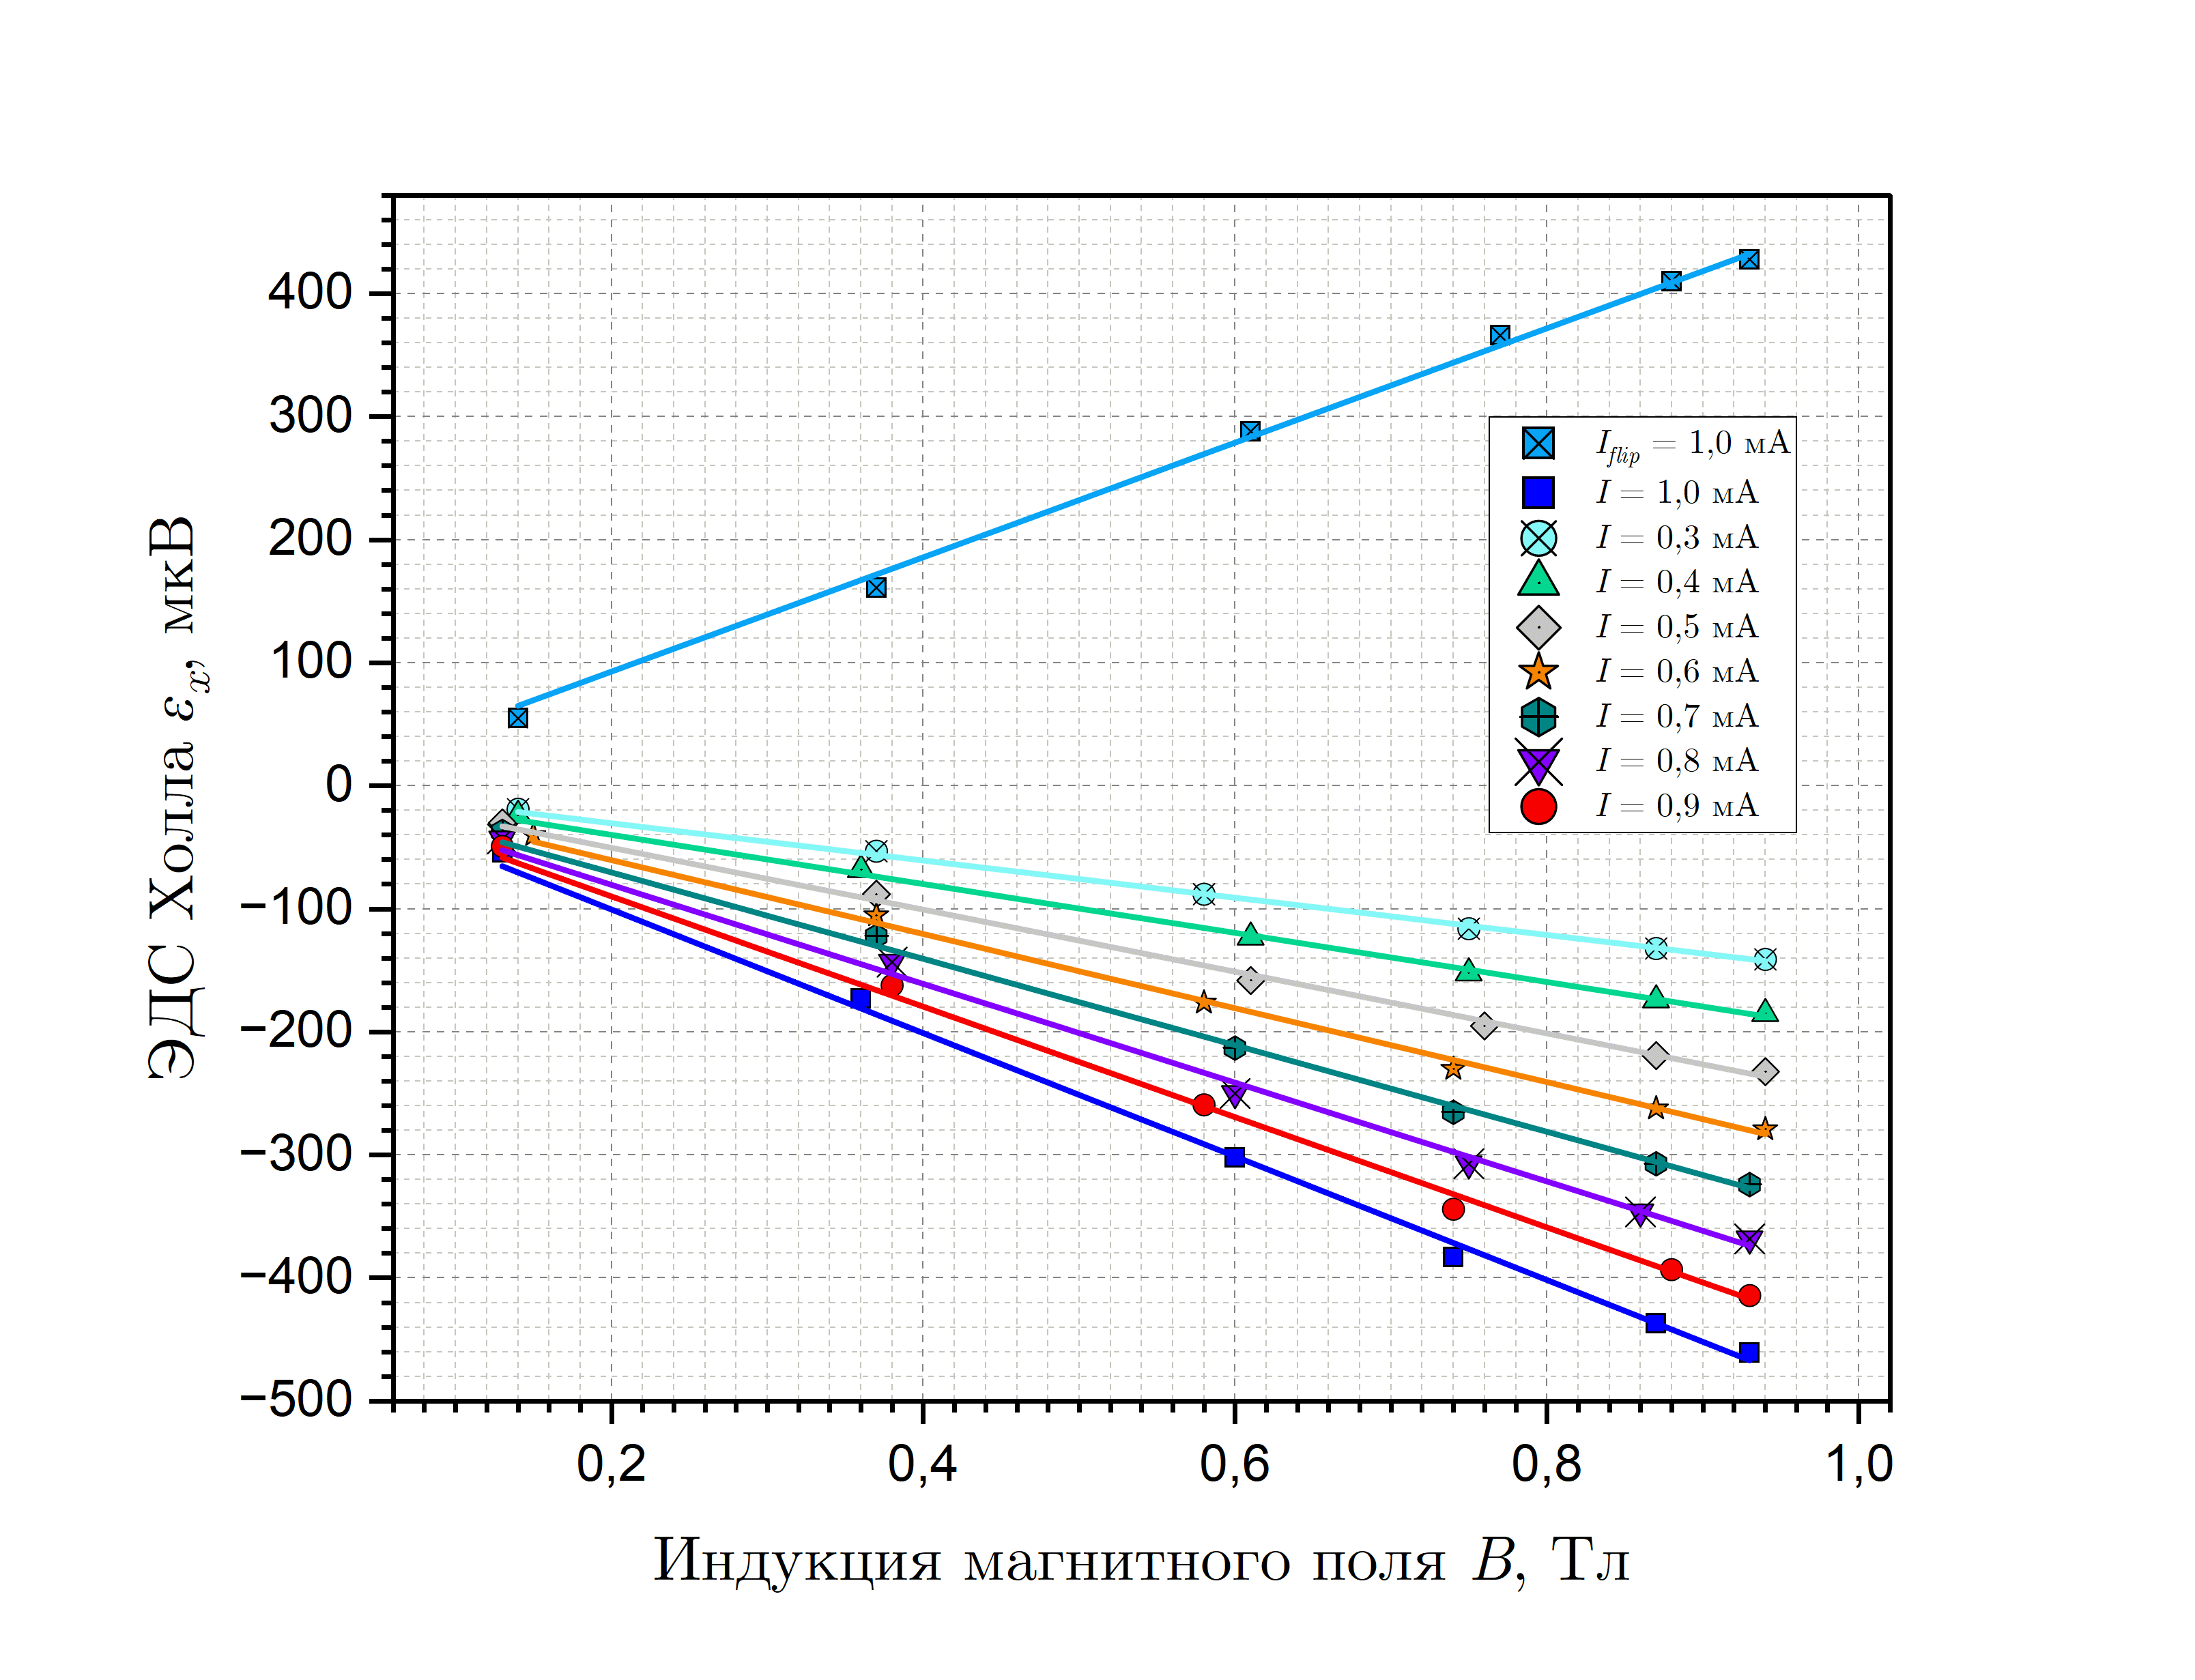
\includegraphics[width = 15 cm]{images/graph_EDS.png}
        \caption{Графики зависимости $\mathcal{E}_x = f(B)$}
        \label{graph:EDS}
    \end{figure}

    Аппроксимируем полученные данные зависимостями вида $\mathcal{E}_x = K(I) \cdot B + const$ при помощи программы \textit{OriginPro 2023b}. Результаты аппроксимации представлены в таблице \ref{table_approx}.

    \begin{table}[H]
        \centering
        \begin{tabular}{|c|c|c|}
        \hline
        $I$, мА & $\lvert K(I) \rvert \cdot 10^{-3}$, В/Тл  & $\sigma_{K(I)} \cdot 10^{-3}$, В/Тл  \\ \hline
        0,3 & 1,51 & 0,01 \\ \hline
        0,4 & 1,99 & 0,02 \\ \hline
        0,5 & 2,51 & 0,03 \\ \hline
        0,6 & 3,00 & 0,03 \\ \hline
        0,7 & 3,51 & 0,04 \\ \hline
        0,8 & 4,02 & 0,05 \\ \hline
        0,9 & 4,48 & 0,05 \\ \hline
        1,0 & 5,02 & 0,05 \\ \hline
        1,0 & 4,65 & 0,05 \\ \hline
        \end{tabular}
        \caption{Результаты аппроксимации зависимостей $\mathcal{E}_x = f(B)$}
        \label{table_approx}
    \end{table}

    По данным таблицы \ref{table_approx} был построен график зависимости $K = f(I)$ (рис. \ref{graph:k}).

    \begin{figure}[H]
        \centering
        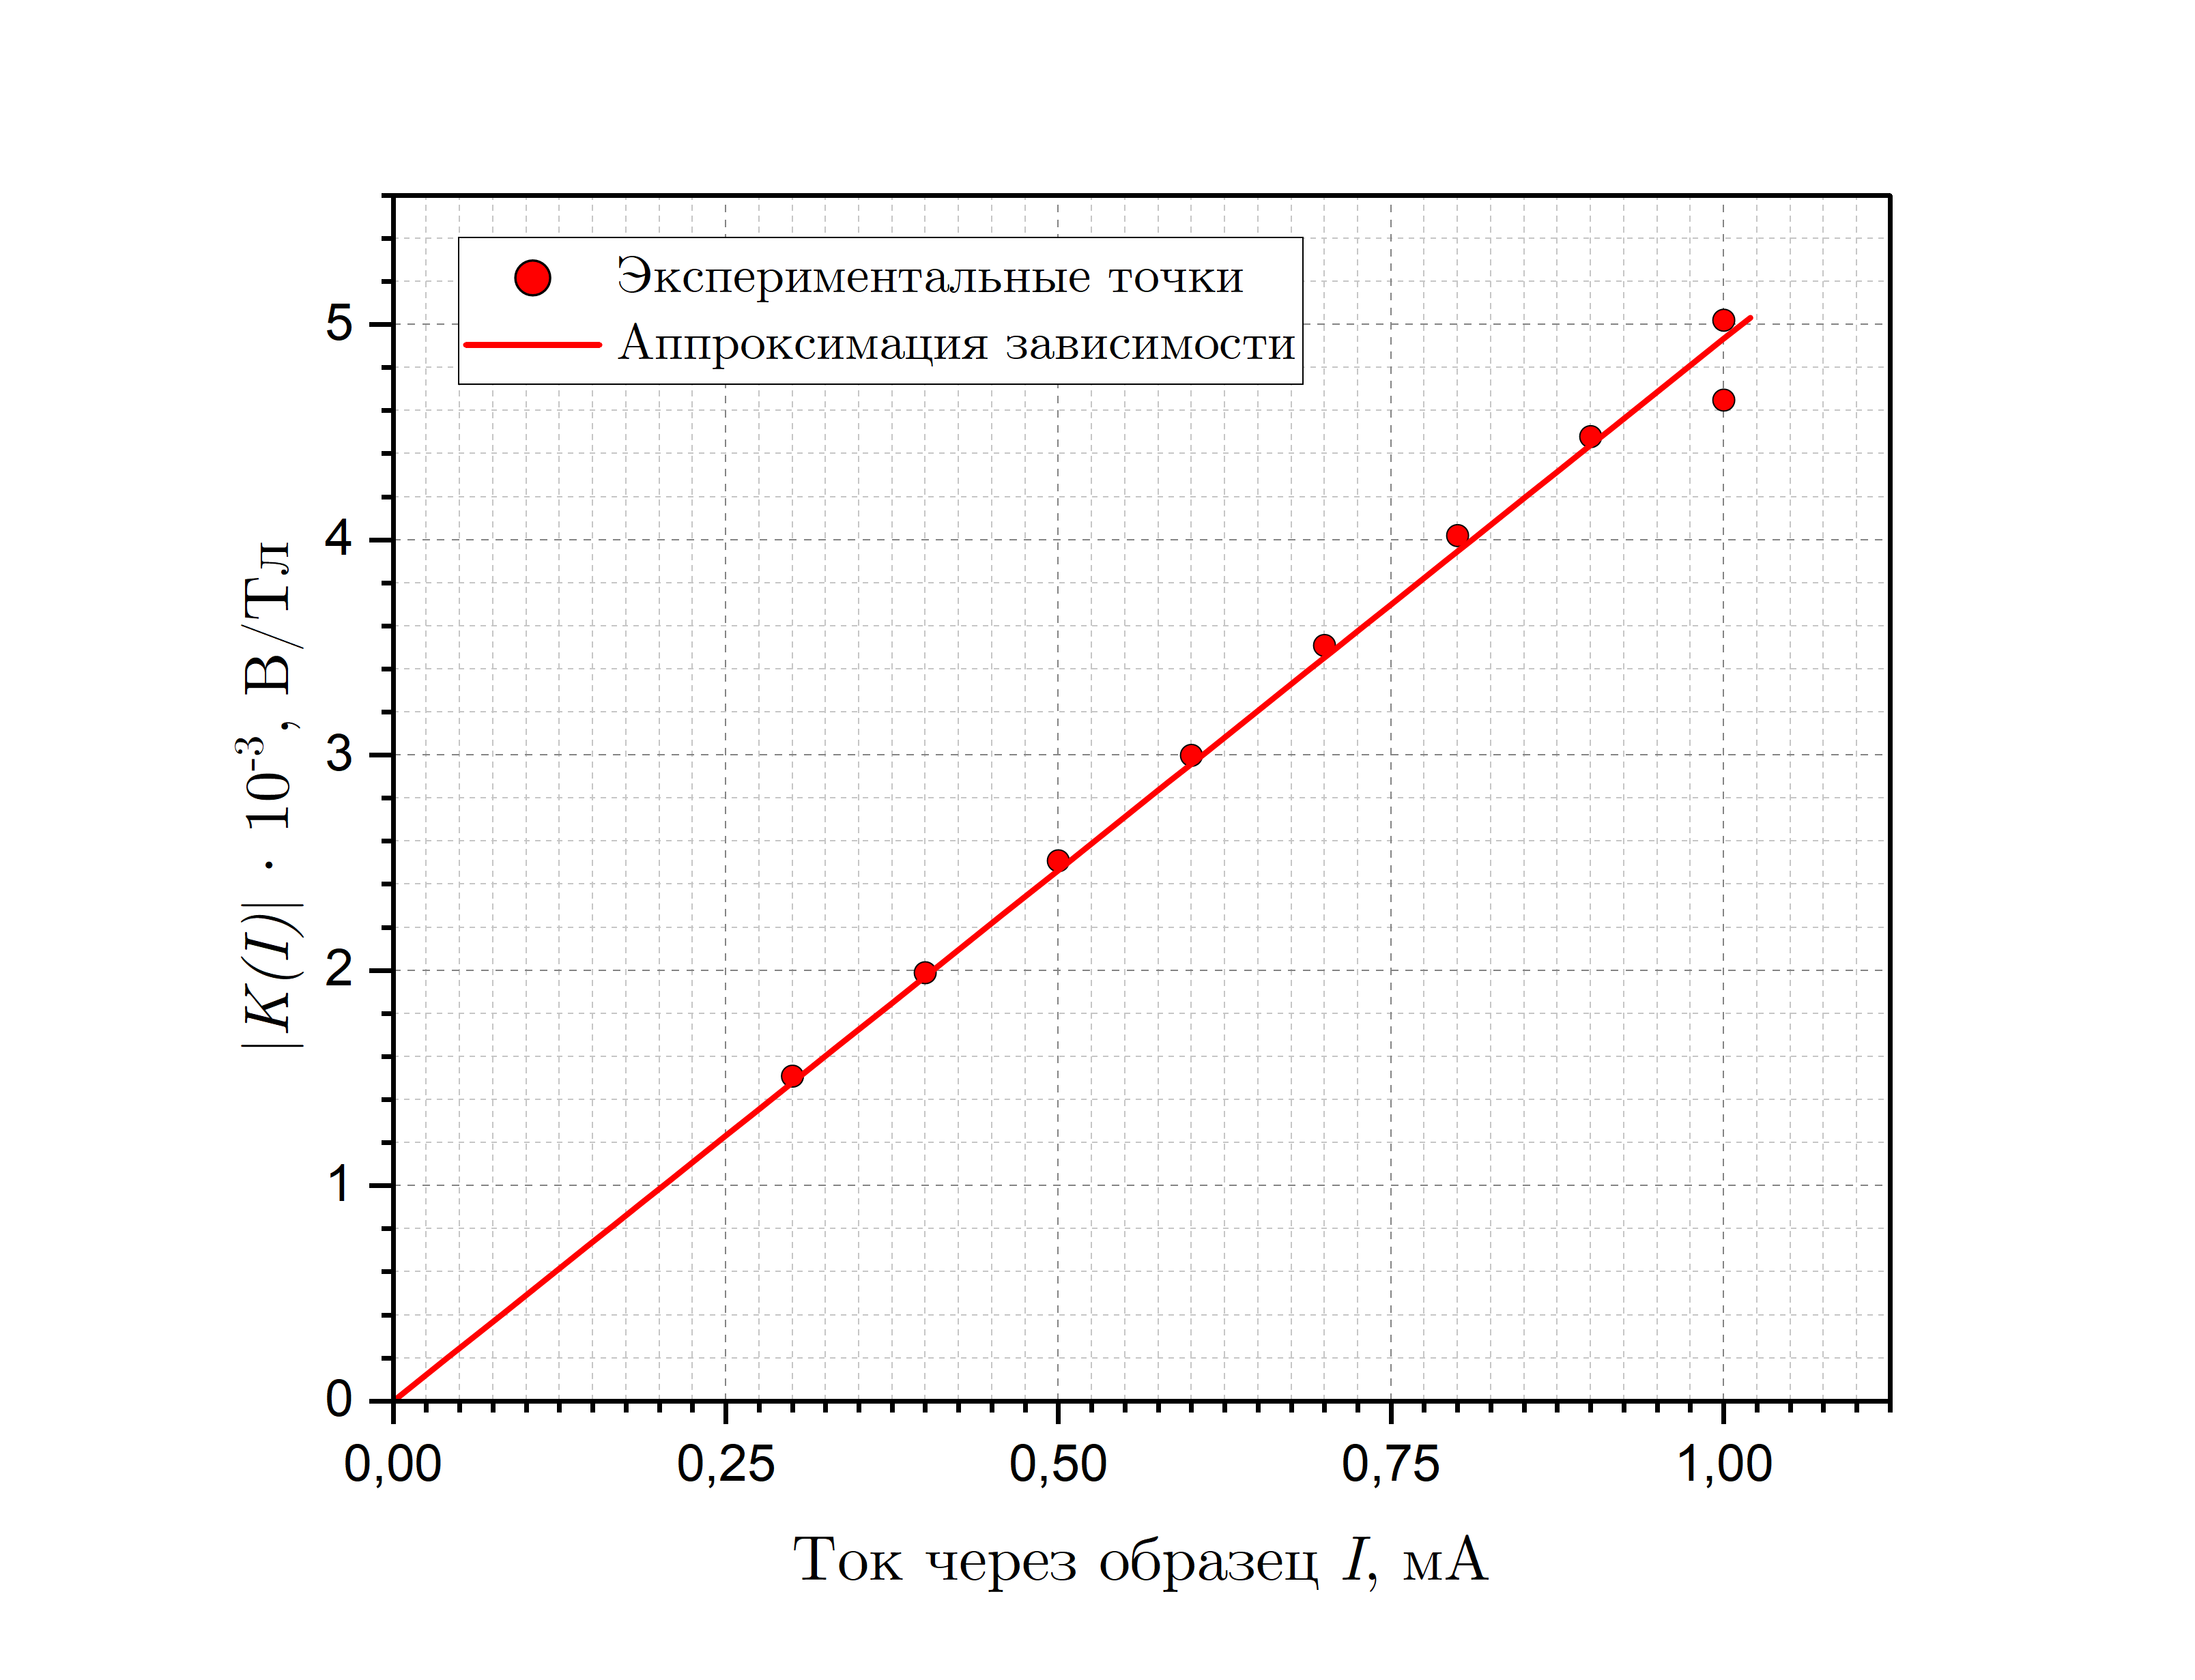
\includegraphics[width = 15 cm]{images/graph_k.png}
        \caption{График зависимости $K(I)$}
        \label{graph:k}
    \end{figure}

     Аппроксимируя полученную зависимость при помощи программы \textit{OriginPro 2023b}, получим

     \begin{equation}
         \frac{\Delta K}{\Delta I} = \left( 4,93 \pm 0,05 \right) \: \frac{\text{В}}{\text{Тл} \cdot \text{А}}.
     \end{equation}

     Тогда, согласно соотношению (\ref{eq_Rx}), $R_x = \frac{\Delta K}{\Delta I} a$, где $a = 1,5$ мм -- толщина исследуемого образца. Окончательно получим

     \begin{equation}
         \boxed{R_x = \left( 7,4 \pm 0,1 \right) \cdot 10^{-3} \: \frac{\text{В} \cdot \text{м}}{\text{Тл} \cdot \text{А}}}.
     \end{equation}

     Отсюда, пользуясь соотношением (\ref{eq_Rx}), получим концентрацию носителей заряда

     \begin{equation}
         n = \left( 0,85 \pm 0,01 \right) \cdot 10^{21} \: \text{м}^{-3} 
     \end{equation}

     \subsection{Расчёт удельной проводимости и подвижности}

     По формуле (\ref{eq_sigma}) была рассчитана удельная проводимость нашего образца. По результатам измерений $U_{35} = 1,784$ мВ, $I = 1$ мА, $L_{35} = 3$ мм и $l = 1,7$ мм. В итоге получаем

    \begin{equation}
        \sigma = \left( 660 \pm 10 \right) \: \text{Ом}^{-1} \cdot \text{м}^{-1}
    \end{equation}
     
    Теперь, зная эти характеристики, можно рассчитать подвижность носителей заряда по следующей формуле

    \begin{equation}
        b = \frac{\sigma}{en} = \left( 4850 \pm 100 \right) \: \frac{\text{см}^2}{\text{В} \cdot \text{с}}
    \end{equation}


    \section{Заключение}

    Результаты работы представлены в таблице \ref{table:result}.

    \begin{table}[H]
        \centering
        \begin{tabular}{|c|c|c|c|l|}
        \hline
        \multirow{2}{*}{\begin{tabular}[c]{@{}c@{}}$R_X \pm \Delta R_X,$ \\ $10^{-3} \cdot \text{м}^3/\text{Кл}$\end{tabular}} & \multirow{2}{*}{Знак носителя} & \multirow{2}{*}{\begin{tabular}[c]{@{}c@{}}$n \pm \Delta n,$ \\ $10^{21} \cdot \text{м}^{-3}$\end{tabular}} & \multirow{2}{*}{\begin{tabular}[c]{@{}c@{}}$\sigma \pm \Delta \sigma,$ \\ $\text{Ом}^{-1} \cdot \text{м}^{-1}$\end{tabular}} & \multirow{2}{*}{\begin{tabular}[c]{@{}c@{}}$b \pm \Delta b,$ \\ $\text{см}^2 \cdot (\text{В} \cdot \text{с})^{-1}$\end{tabular}} \\
        &  &  &  &  \\ \hline
        \multirow{2}{*}{\begin{tabular}[c]{@{}c@{}}$\left( 7,4 \pm 0,1 \right)$\end{tabular}} & \multirow{2}{*}{$-$} & \multirow{2}{*}{\begin{tabular}[c]{@{}c@{}}$\left( 0,85 \pm 0,01 \right)$\end{tabular}} & \multirow{2}{*}{\begin{tabular}[c]{@{}c@{}}$\left( 660 \pm 10 \right)$\end{tabular}} & \multirow{2}{*}{\begin{tabular}[c]{@{}c@{}}$\left( 4850 \pm 100 \right)$\end{tabular}} \\
        &  &  &  &  \\ \hline
        \end{tabular}
        \caption{Результаты лабораторной работы}
        \label{table:result}
    \end{table}

    Полученные результаты совпали с табличными по порядку. Например, полученная подвижность электронов в германии отличается от табличной ($b_\text{табл} = 3900 \: \text{см}^2 \cdot (\text{В} \cdot \text{с})^{-1}$). Это может свидетельствовать о наличии примесей в исследуемом образце. Также ощутимый вклад в погрешность полученных данных могла внести зависимость характеристик исследуемого образца от температуры, которая могла значительно изменяться вследствие прохождения через образец электрического тока.

\end{document}